% !TeX encoding = UTF-8
% !TeX spellcheck = en_US

\documentclass[
	paper=A4,
	parskip=full,
	chapterprefix=true,
	12pt,
	headings=normal,
	bibliography=totoc,
	listof=totoc,
	titlepage=on,
]{scrreprt}

\usepackage{../../lieb}

\usepackage{feynmp}
\DeclareGraphicsRule{.1}{mps}{*}{}

\graphicspath {{../images/}}

\heads{RWTH Aachen \\ Particle Phyics Lab}{T17 \\ W-Boson}{Lieb | Stettner \\ \today} 
\date{\today}

\newcommand{\MET}{\ensuremath{{\slashed{E}_\mathrm{T}}}\xspace}
\newcommand{\ELET}{\ensuremath{{E_\mathrm{T}^\mathrm{el}}}\xspace}
\newcommand{\MPT}{\ensuremath{{\slashed{p}_\mathrm{T}}}\xspace}
\newcommand{\ELPT}{\ensuremath{{p_\mathrm{T}^\mathrm{el}}}\xspace}
\newcommand{\MT}{\ensuremath{{m_\mathrm{T}}}\xspace}
\newcommand{\MW}{\ensuremath{{m_\mathrm{\PW}}}\xspace}
\newcommand{\MZ}{\ensuremath{{m_\mathrm{\PZ}}}\xspace}
\newcommand{\NC}{\ensuremath{N_\mathrm{C}}\xspace}
\newcommand{\weinberg}{\ensuremath{\theta_\mathrm{W}}\xspace}
\newcommand{\Gammaff}{\ensuremath{\Gamma_\mathrm{\Pfermion \Pfermion}}\xspace}
\newcommand{\GammaW}{\ensuremath{\Gamma_\mathrm{\PW}}\xspace}

\newcommand{\thirdwidth}{0.32\textwidth}
\newcommand{\halfwidth}{0.48\textwidth}
\newcommand{\fullwidth}{1.0\textwidth}

\setlength\parindent{0pt}
\setlength{\parskip}\medskipamount

\title{Particle Physics Laboratory Class \\ \quad \\ Experiment T17 | W-Boson }
\author{Jonas Lieb (312136) \\ Jöran Stettner (312169) \\ \\  RWTH Aachen}

\newcommand{\dnull}{D0\xspace}

\begin{document}

\maketitle

\cleardoublepage

\setcounter{tocdepth}{2}
\tableofcontents

\cleardoublepage

\chapter{Introduction}

This analysis deals with \PW boson physics conducted at the \dnull experiment at the Tevatron accelerator (FERMILAB, Chicago). The dataset has been taken in proton-antiproton collisions at a center-of-mass energy of $\sqrt{s} = \SI{1960}{\giga\electronvolt}$\cite{HBK+2013Experiment}.

\section{Units}
In this report, a natural unit system of particle physics is used: first, the speed of light and Planck's constant are fixed:
\begin{equation}
c \defeq \num{1},\quad \hbar \defeq \num{1}
\end{equation}
From this convention, many quantities arise in units of energy. Additionally, the gigaelectronvolt (\si{\giga\electronvolt}) is chosen as basic energy unit, in order to deal with numbers of magnitude $\order{1}$.

\section{\PW Boson Production and Decay}
The process of interest is the \PW boson production from the valence quarks of the protons and antiprotons, and the decay into an electron and an electron neutrino.
\begin{equation}
	\Pproton\APproton \rightarrow \PWminus \rightarrow \Pelectron + \APnue
\end{equation}
Equivalently, there exists a oppositely charged process:
\begin{equation}
\Pproton\APproton \rightarrow \PWplus \rightarrow \Ppositron + \Pnue
\end{equation}
With the assumption that the \PWplus and \PWminus have the same properties (except the electric charge), one does not expect any difference between the processes. Because of that, the presented analysis will not differentiate between them and treat positrons as electrons in the final state.

Both processes combined have an expected cross section\cite{HBK+2013Experiment} of 
\begin{equation}
	\sigma_\mathrm{theo} = \SI{2.58 +- 0.09}{\nano\barn}
	\label{eq:theoretical_cross_section}
\end{equation}
and should show a resonance at the predicted \PW-Boson mass\cite{Oo2014Review} of 
\begin{equation}
	% don't use the macro here
	m_\mathrm{\PW}^\mathrm{theo} = \SI{80.385 +- 0.015}{\giga\electronvolt}
\end{equation}

\section{The \dnull Detector}
The measurement took place in 2004 until 2006 at the \dnull experiment at FERMILAB. The \dnull detector is a cylindrical particle detector located around the Tevatron beam pipe. It consist of a silicon tracker in the center region, enclosed by an Argon electromagnetic calorimeter.

Inside the detector, a Cartesian coordinate system and a cylindrical coordinate system are used. The origin of both systems lies in the interaction point, with the z-axis pointing along the beam pipe. The angle $\phi$ is measured in a plane perpendicular to the z-axis. 

Because the colliding protons are composite particles, the longitudinal momentum of the interacting quarks is unknown. The transversal components, however, are zero in the initial state. From momentum conservation it follows that the sum of all transversal momenta in the final state is also zero. 
To represent this conservation in the transversal plane, energies and momenta are projected onto it. This introduces the transverse electron energy \ELET.
Another important quantity is the missing transverse energy \MET which is calculated as negative sum of all particles momenta, projected onto the transverse plane.


\chapter{Monte-Carlo Samples}
\label{ch:mc_samples}

\section{Reweighting}
The final goal of this experiment is to perform a template fit between distributions of simulated Monte Carlo (MC) events and measured data, in order to find the \PW-Boson mass \MW. For the template fit, multiple MC distributions are necessary, one for each hypothetical \PW boson mass. Since MC simulations are computation intensive, an alternative approach is used: the actual simulation has only been performed once, but each MC event additionally contains a set of \num{19} weights, which correspond to different hypothetical \PW masses in the range of \SIrange{79.9446}{80.8446}{\giga\electronvolt} (for a complete reference, see the appendix of \cite{HBK+2013Experiment}). When aggregating distributions, each event has to be counted with the weight of the \PW mass of interest.

\begin{figure}
	\centering
	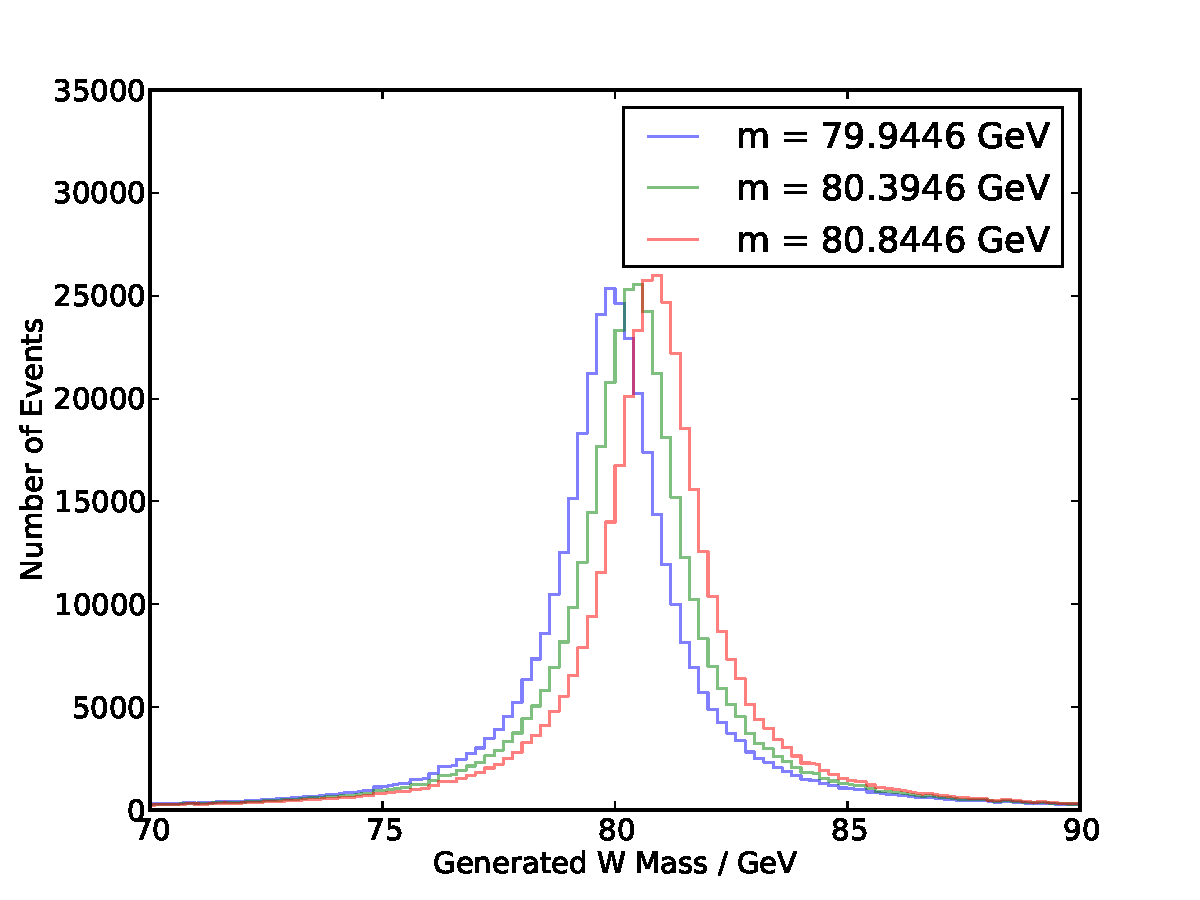
\includegraphics{mc_examples}
	\caption{Histogram of \PW masses. Shown is the generator \PW mass, which is stored inside the MC events, reweighted for three different example masses. One can observe the expected Breit-Wigner distribution, with the centers shifted.}
	\label{fig:mc_examples}
\end{figure}

Figure \ref{fig:mc_examples} shows the result of the reweighting: For this plot, the "true" \PW mass has been obtained from the Monte Carlo generator data. The histogram has been filled with the generator mass and the weights corresponding to the \PW masses \SI{79.9446}{\giga\electronvolt}, \SI{80.3946}{\giga\electronvolt} and \SI{80.8446}{\giga\electronvolt}. The illustration shows that the reweighting approach is valid, although the weights only change the plot along the vertical axis, the overall Breit-Wigner curve has shifted to different masses.

\section{Scaling}
Of course, only a limited amount of measured data is available. The integrated luminosity of the dataset sample\cite{HBK+2013Experiment} is:
\begin{equation}
	\mathcal{L_\mathrm{data}} = \SI{198 +- 20}{\per\pico\barn}
\end{equation}
Opposed to this, $N_\mathrm{gen} = \num{1164699}$ Monte Carlo events have been generated. An intuitive way to compare the number of MC events to the number of data events is to construct a "MC luminosity". For this, the theoretical cross section from equation \ref{eq:theoretical_cross_section} is used to predict the luminosity corresponding to $N_\mathrm{gen}$ events. Here and in the following equations (if not stated otherwise), Gaussian error propagation is used:
\begin{equation}
	\mathcal{L}_\mathrm{MC} = \frac{N_\mathrm{gen}}{\sigma_\mathrm{theo}} = \SI{451 +- 16}{\per\pico\barn}
\end{equation}
This shows that for a comparison between data and MC, the number of MC events has to be scaled down by a factor of $\approx \num{2.3}$. Curiously enough, the lab manual suggests an additional correction factor of $\mathrm{corr} = \num{0.90 +- 0.10}$ of unknown origin.
Combined, the weight for each MC event (not including the shape-reweighting) is:
\begin{equation}
	w = \frac{\mathcal{L}_\mathrm{data}}{\mathcal{L}_\mathrm{MC}} \cdot \mathrm{corr} = \mathcal{L}_\mathrm{data} \cdot \frac{\sigma_\mathrm{theo}}{N_\mathrm{gen}} \cdot \mathrm{corr} = \num{0.395 +- 0.061}
	\label{eq:reweighting_total}
\end{equation}
From this, all MC events counts can be reweighted:
\begin{equation}
	N_\mathrm{MC}' = w \cdot N_\mathrm{MC} = \frac{\mathcal{L}_\mathrm{data}}{\mathcal{L}_\mathrm{MC}} \cdot \mathrm{corr} \cdot N_\mathrm{MC}
\end{equation}


\chapter{Selection of Events}
In this chapter, the measured variables are presented and the selection of events is explained. \\
The distributions of the measured and simulated quantities are shown in figures \ref{fig:no_cuts_Et},\ref{fig:no_cuts_met}, \ref{fig:no_cuts_eta}, \ref{fig:no_cuts_dphi}, \ref{fig:no_cuts_dz} and \ref{fig:no_cuts_iso}. The histogram labeled "MC (all)" contains all simulated events for the weight $\MW = \SI{80.3946}{\giga\electronvolt}$. The small component of \Ptau leptons is plotted separately as "MC (tau only)" to point out its contribution. It becomes clear that the MC-generator did not simulate all processes which occur in the detector, see for example the double-bump structure in the distribution of transverse electron energy. To perform the analysis which is based on a template fit, it is important to select only those events which fall in regions where data and MC are in good agreement. Otherwise, a discrepancy coming from background processes or missing simulation would be interpreted as a mismatch to the simulated \PW mass. Among others, occurring background processes are: 
\begin{itemize}
	\item $\Ppizero \rightarrow 2 \Pphoton$ decays which could account for the lower electron energies if the $\gamma$ is misidentified.
	\item Jets which are misidentified as electrons. The electron isolation variable becomes smaller in this case.
	\item $\PZ \rightarrow \Ppositron \Pelectron$ decays where one of the leptons leaves the detector unnoticed.
	\item $\tau \rightarrow e+\bar{\nu_e}+\nu_{\tau}$ (also simulated in MC)
\end{itemize}

To constrain the analysis to regions of good agreement between MC and data, the following cuts are applied to all events:
\begin{table}[htbp]
	\centering
	\begin{tabular}{ 
			l 
			l
			l
			l
		}
		\toprule
		{Quantity} & {Threshold} & {Motivation} \\ 
		\midrule
		\MET & $>\SI{20}{\giga\electronvolt}$ & Beginning of background-dominated region \\
		\ELET & $>\SI{30}{\giga\electronvolt}$ & No low energy electrons (e.g. \Ppizero) \\
		Electron Isolation & $< \num{0.03}$ & Reject misidentified Jets \\
		$\Delta \phi\left(\MET,\ELET\right)$ & $> \num{2.85}$ & Expected back-to-back events, $\Delta \phi \approx \pi$ \\
		$\Delta z\left(\MET,\ELET\right)$ & $<\SI{0.2}{\milli\meter}$ & Short lifetime of the \PW boson, no offset expected \\
		
		\bottomrule
	\end{tabular}
	\caption{Applied cuts and short Motivation.}
	\label{tbl:cuts_summary}
\end{table}

\begin{figure}
	\centering
	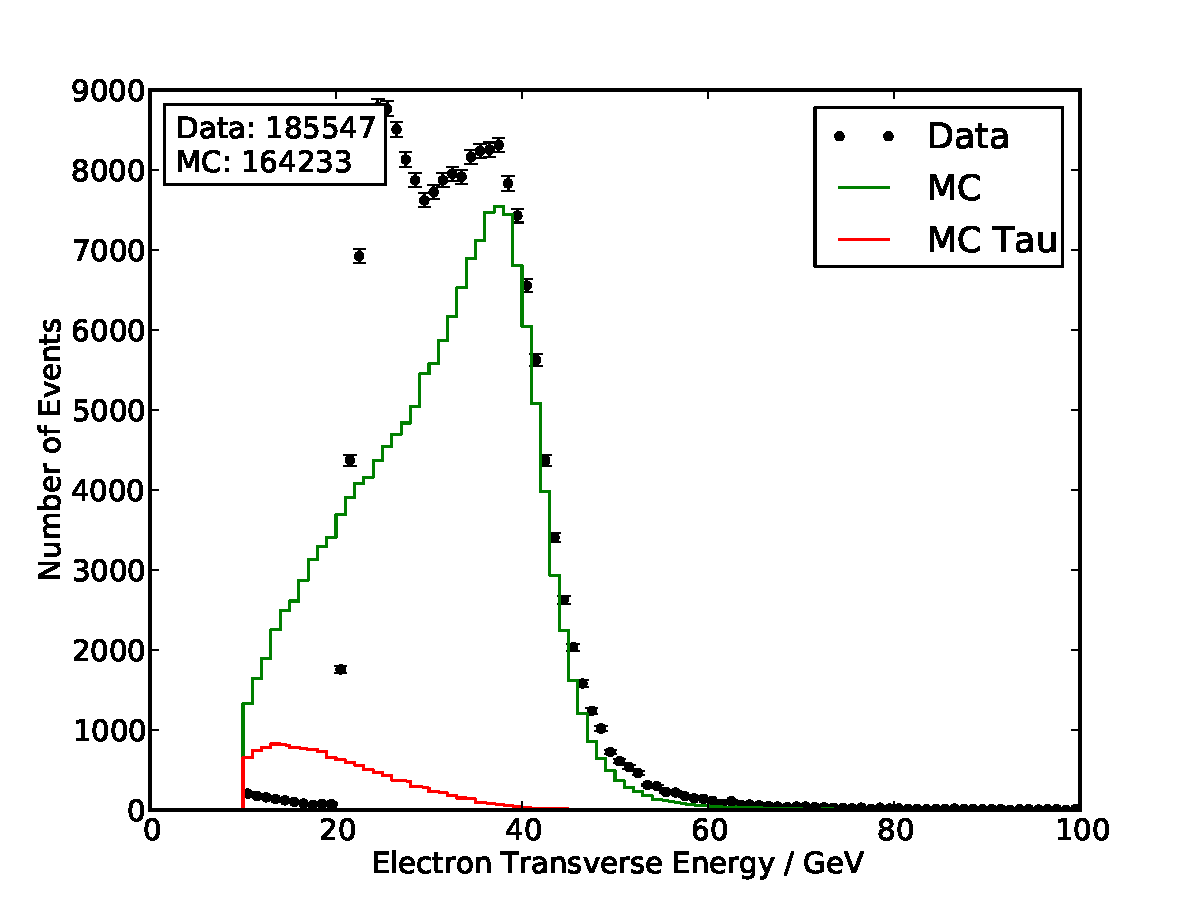
\includegraphics[width=0.9\textwidth]{nocuts/E_T_el}
	\caption{Transverse Electron Energy measured in the Central Calorimeter.}
	\label{fig:no_cuts_Et}
\end{figure}
\begin{figure}
	\centering
	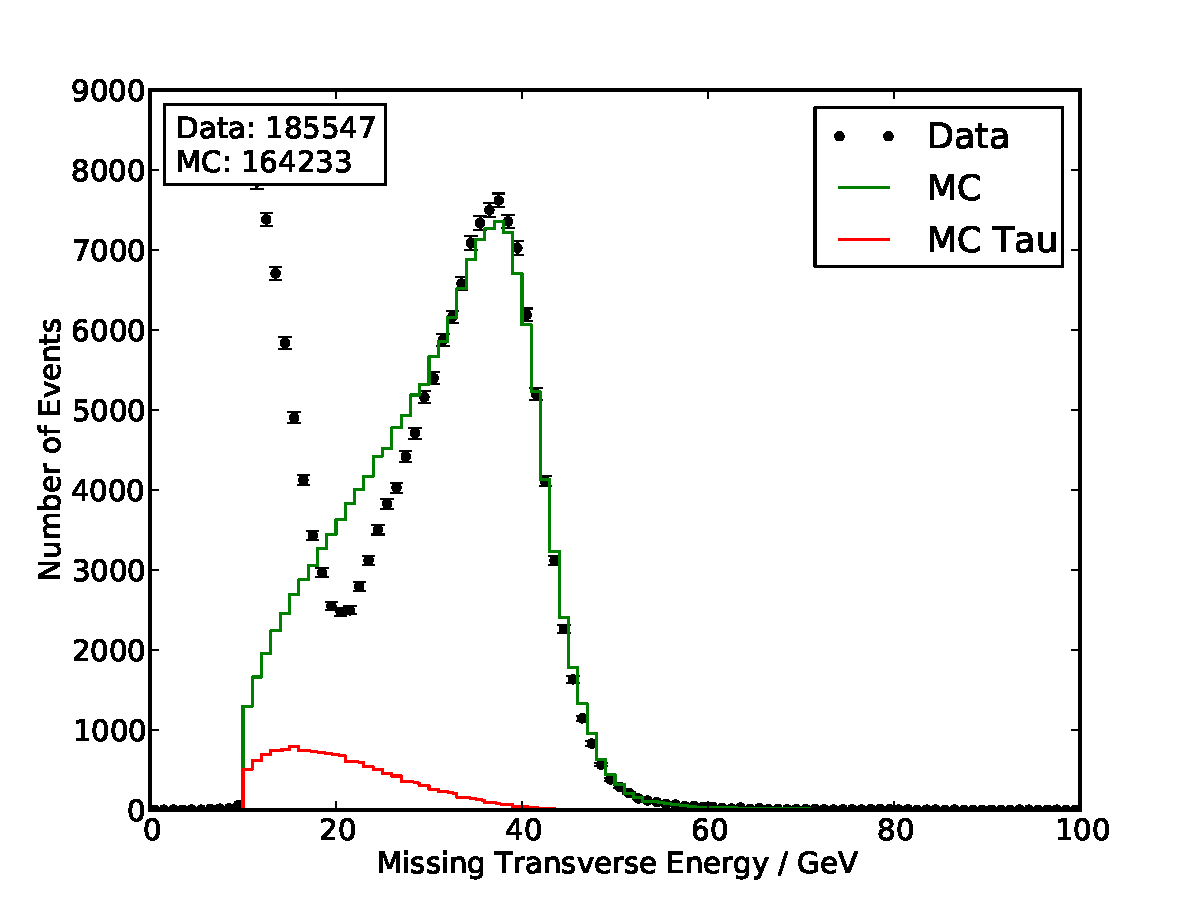
\includegraphics[width=0.9\textwidth]{nocuts/E_T_miss}
	\caption{Missing Transverse Energy, calculated using the constraint of momentum conservation in the transversal plane.}
	\label{fig:no_cuts_met}
\end{figure}

\begin{figure}
	\centering
	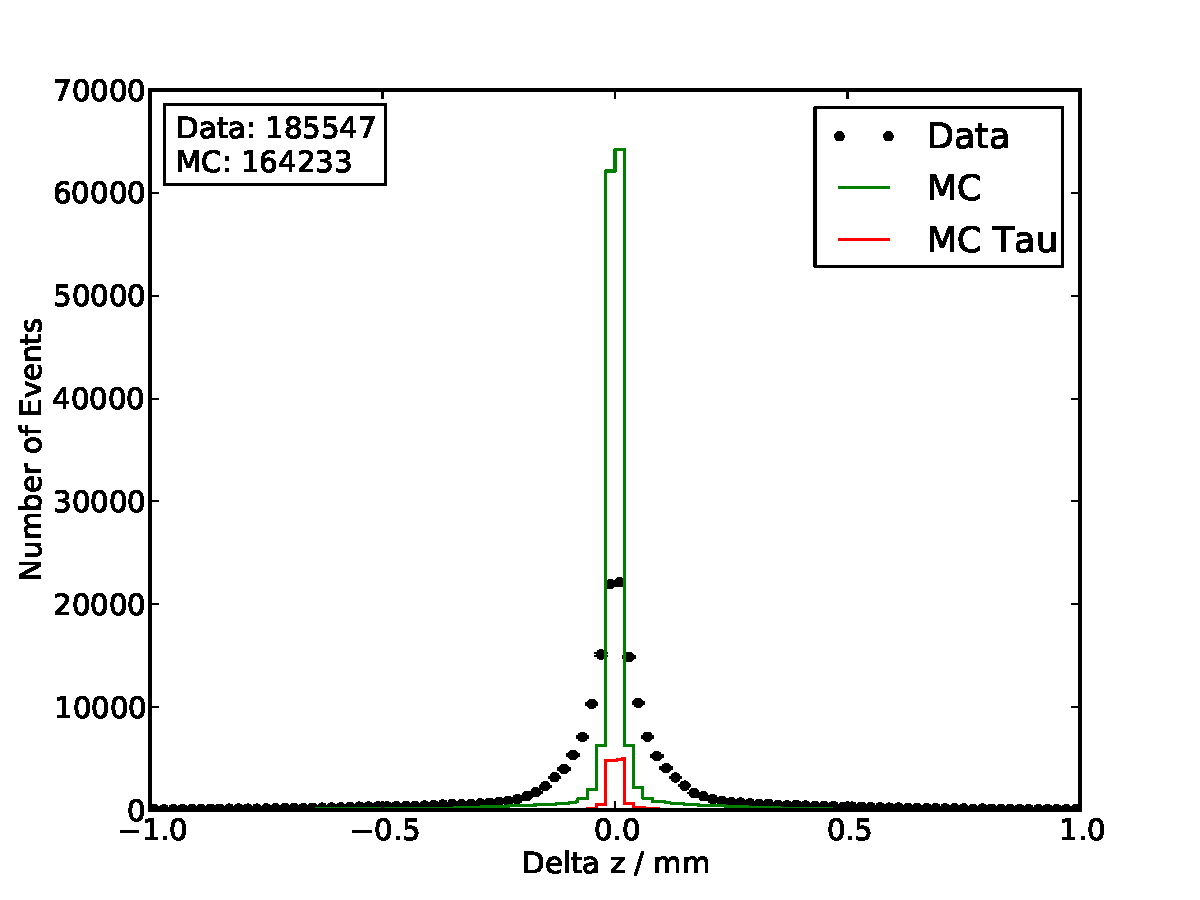
\includegraphics[width=0.9\textwidth]{nocuts/delta_z}
	\caption{Distribution of the distance between the origin of \MET and the electron track.}
	\label{fig:no_cuts_dz}
\end{figure}
\begin{figure}
	\centering
	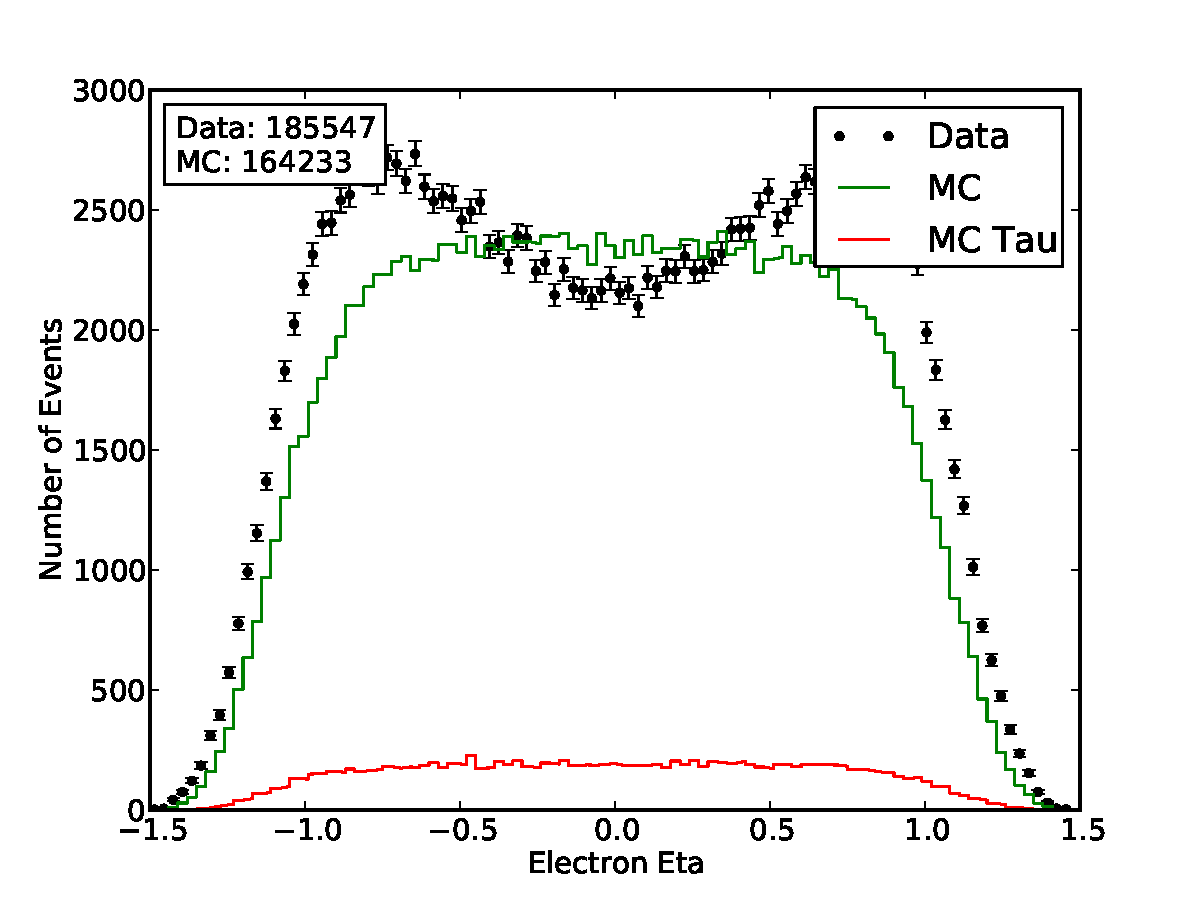
\includegraphics[width=0.9\textwidth]{nocuts/eta_el}
	\caption{Distribution of the Pseudorapidity of the Electron showing discrepancies between the measured data and MC.}
	\label{fig:no_cuts_eta}
\end{figure}

\begin{figure}
	\centering
	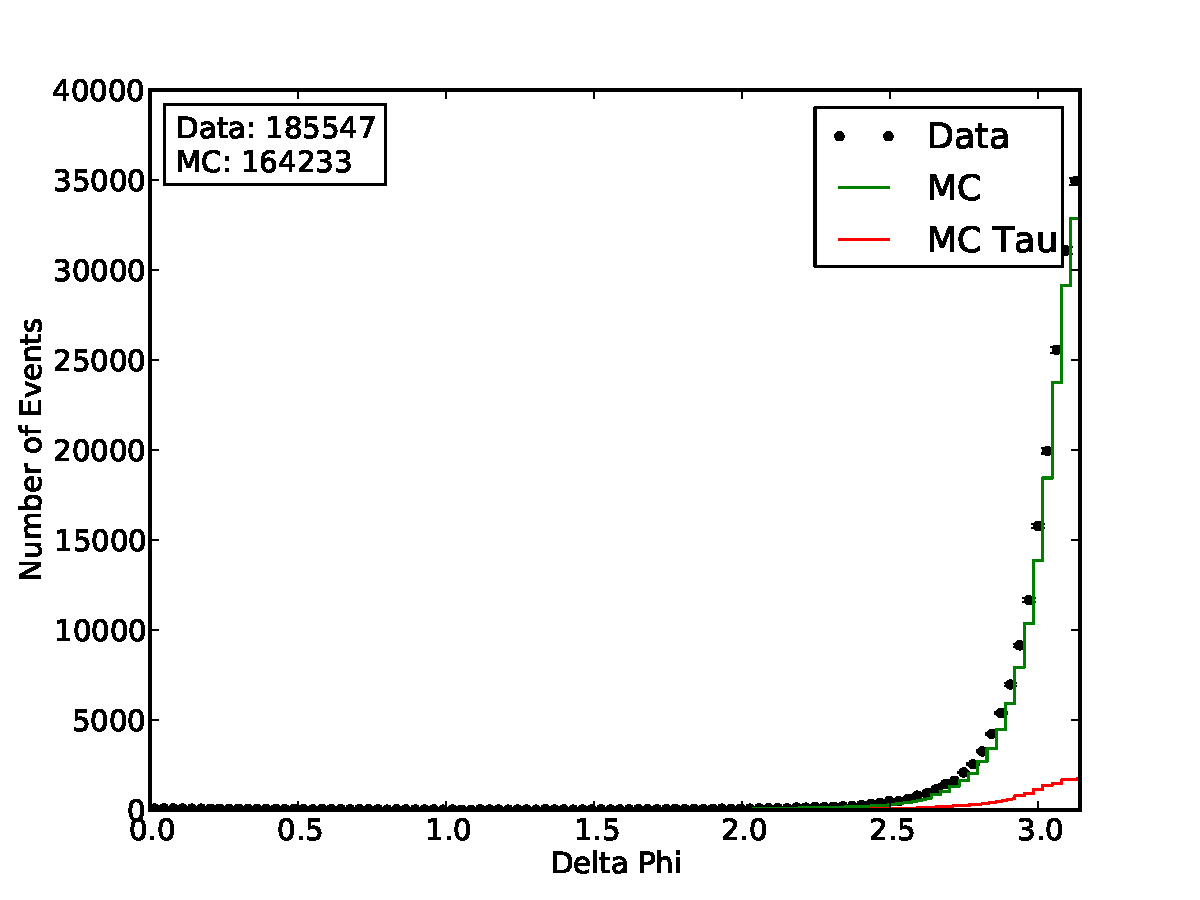
\includegraphics[width=0.9\textwidth]{nocuts/delta_phi}
	\caption{Distribution of the difference in Polar Angle $\phi$ between the directions of MET and the electron.}
	\label{fig:no_cuts_dphi}
\end{figure}
\begin{figure}
	\centering
	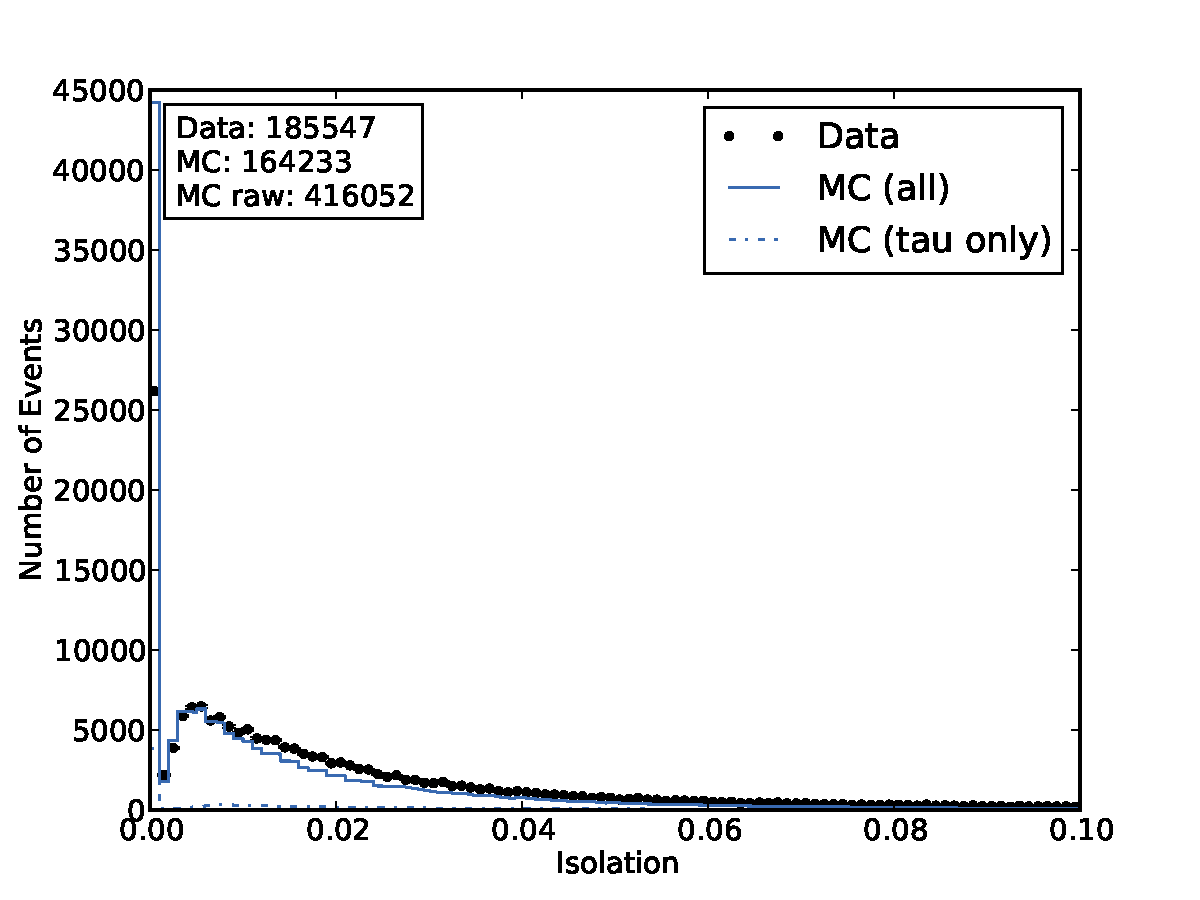
\includegraphics[width=0.9\textwidth]{nocuts/el_iso}
	\caption{Distribution of the isolation variable describing the tidiness in the vicinity of the electron's impact in the EM calorimeter}
	\label{fig:no_cuts_iso}
\end{figure}

\FloatBarrier

After applying these cuts, the agreement between data and MC becomes much better as can be seen in the distribution of the transverse electron energy (see figure \ref{fig:cuts_Et}). Since the reconstruction of the neutrino is only possible in the transverse plane of the detector, the invariant mass of the \PW boson can not be calculated directly. The following analysis is therefore based on the transverse mass, which is calculated from the transverse momentum of the electron $p_T^\mathrm{el}$ and the missing transverse momentum $\slashed{p}_T$ for each event:
\begin{equation}
	\MT \defeq \sqrt{\left(\MPT+\ELPT\right)^2} = \sqrt{\MET \ELET (1-\cos{\Delta \phi})}
\label{eq:m_t}
\end{equation} 
The distribution of this quantity is shown in figure \ref{fig:cuts_Mt} and shows good agreement after applying the described cuts. Since rescaling of the MC events to the luminosity of the data sample as described in chapter \ref{ch:mc_samples} is very uncertain, the agreement of the absolute height is not very good. This discrepancy will not influence the main goal of the analysis and is therefore not investigated further. 


\begin{figure}
	\centering
	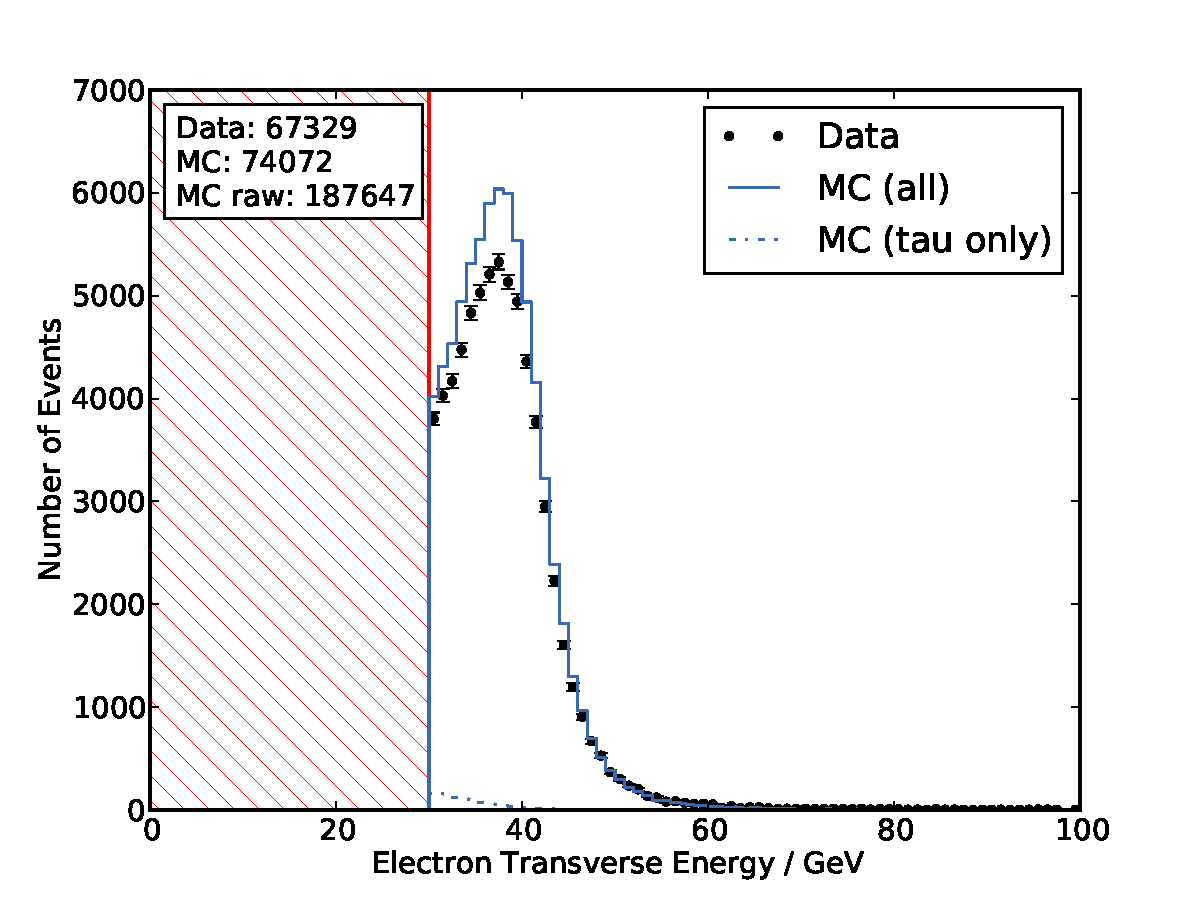
\includegraphics[width=0.9\textwidth]{allcuts/E_T_el}
	\caption{Transverse Electron Energy, all cuts applied.}
	\label{fig:cuts_Et}
\end{figure}
\begin{figure}
	\centering
	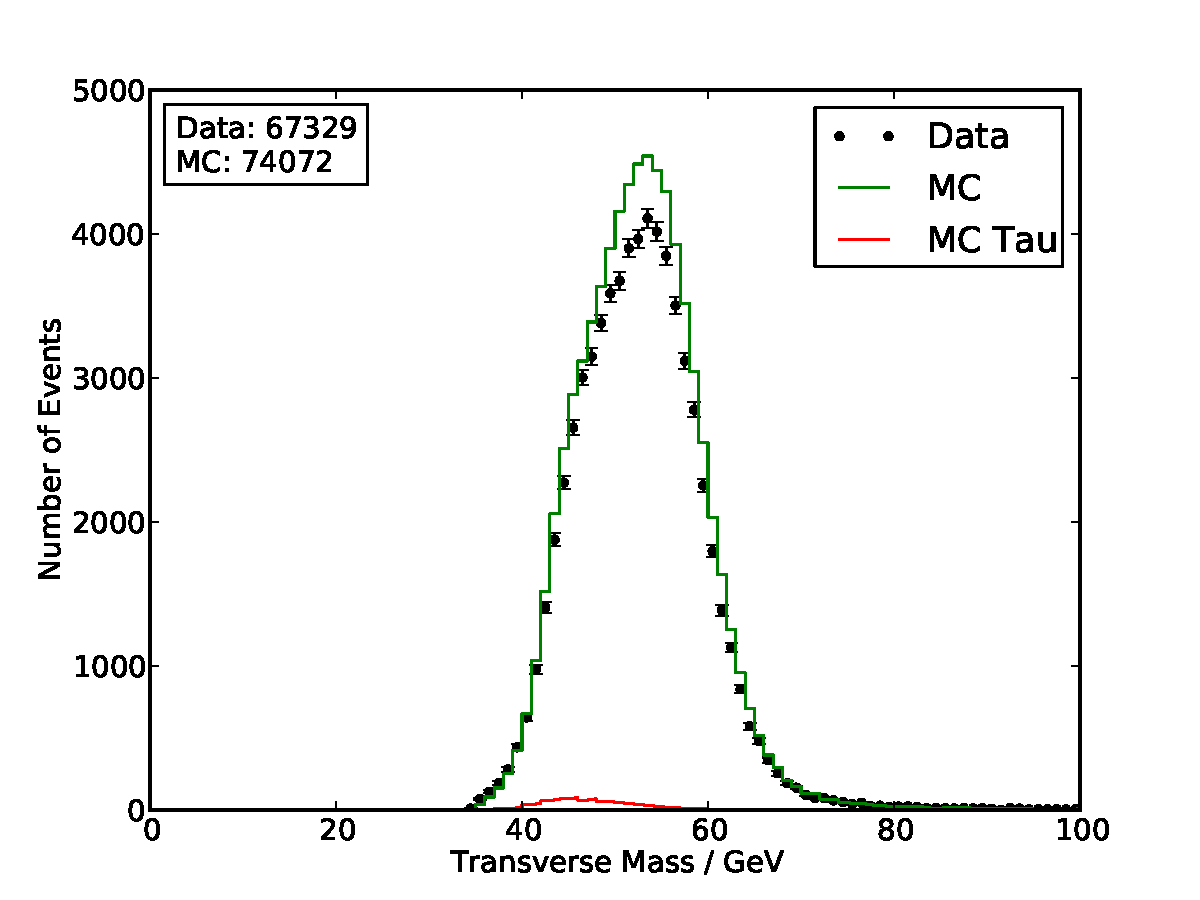
\includegraphics[width=0.9\textwidth]{allcuts/m_T}
	\caption{Reconstructed Transverse Mass, all cuts applied.}
	\label{fig:cuts_Mt}
\end{figure}

\chapter{Determination of the Process Cross Section}
To determine the process cross section $\sigma_\mathrm{data}$ from the data, the lab manual poses a complex formula:
\begin{equation}
	N_\mathrm{data} = \mathrm{eff} \cdot \mathrm{corr} \cdot \sigma_\mathrm{data} \cdot \mathcal{L}_\mathrm{data}
	\label{eq:data_xsec}
\end{equation}
Here, the efficiency $\mathrm{eff}$ contains detector efficiency and acceptance as well as analysis efficiency (e.g. cuts) and is the only unknown factor in this equation. The correction factor $\mathrm{corr}$ and data luminosity $\mathcal{L}_\mathrm{data}$ are defined according to chapter \ref{ch:mc_samples}, $N_\mathrm{data}$ is the number of event after the application of all cuts.

The efficiency can be determined by executing the analysis on the entire Monte Carlo dataset and comparing this to the initial number of generated events, $N_\mathrm{gen}$:
\begin{equation}
	\mathrm{eff} = \frac{N_\mathrm{MC}}{N_\mathrm{gen}}
\end{equation}

Substitution back into equation \ref{eq:data_xsec} and combining this result with \ref{eq:reweighting_total} yields:
\begin{equation}
	N_\mathrm{data} = \frac{N_\mathrm{MC}}{N_\mathrm{gen}} \cdot \mathrm{corr} \cdot \mathcal{L}_\mathrm{data} \cdot \sigma_\mathrm{data} = \frac{N_\mathrm{MC} \cdot w}{\sigma_\mathrm{theo}} \cdot \sigma_\mathrm{data}
\end{equation}
This gives the final equation for the cross section
\begin{equation}
	\sigma_\mathrm{data} = \frac{N_\mathrm{data}}{N_\mathrm{MC} \cdot w} \cdot \sigma_\mathrm{theo}
\end{equation}

Here, the rescaled number of MC events from chapter \ref{ch:mc_samples} can be reused. The formula is plausible, since for a perfect MC simulation $N_\mathrm{data} = N_\mathrm{MC}'$ and thus $\sigma_\mathrm{data} = \sigma_\mathrm{theo}$.

The measurement can be read off from figure \ref{fig:cuts_Mt}:
\begin{equation}
	N_\mathrm{MC} = \num{187647}, \quad
	N_\mathrm{data} = \num{67329 +- 259} 
\end{equation}
Here, the conventional Poission error of $\sigma_N = \sqrt{N}$ is used for the data, which is valid for $N \gg 1$ (fulfilled in this case).
The total cross section is then:
\begin{equation}
	\sigma_\mathrm{data} = \frac{\num{67329 +- 259}}{\num{187647} \cdot (\num{0.395 +- 0.061})} \cdot \SI{2.58 +- 0.09}{\nano\barn} = \SI{2.35 +- 0.35}{\nano\barn}
\end{equation}

This formula also directly shows the comparison between theoretical prediction and this measurement. The factor between both values is \begin{equation}
	\frac{N_\mathrm{data}}{N_\mathrm{MC} \cdot w} = \num{0.909 +- 0.140}
\end{equation} 
Although this results is slightly lower than the theoretical expectation, the measurements are compatible within their errors.

The largest error sources on this method are the determination of the measured luminosity $\mathcal{L}_\mathrm{data}$ and the odd correction factor $\mathrm{corr}$, both contribute a relative uncertainty of \SI{10}{\percent} each. The error on the theoretical value and the statistical uncertainty on $N_\mathrm{data}$ are negligible.

\chapter{Determination of the \PW Boson Mass}
The central analysis of this experiment is the determination of the \PW boson mass in a template fit. The idea is to extract the correct \PW mass from the distribution of measured quantities like the transverse mass by comparing it to the generated MC-datasets. 


\section{Renormalization of the MC dataset}
Since the information of the \PW mass is fully contained in the shape, the MC-datasets are rescaled again in this part of the analysis. By normalizing them to the total number of data events, the unpleasant correction factor is not needed anymore and the absolute height matches much better between Data and MC. The rescaling is done by the modified weighting factor, which is applied to the MC events:
\begin{equation}
w_{\mathrm{normalize}}=\frac{N_{\mathrm{data}}}{N_{\mathrm{MC}}}
\end{equation}

\section{Binning}
The bin width is chosen by visual inspection. There are multiple criteria that have to be fulfilled for a reasonable bin width: each bin has to contain a large number of events ($N^i_\mathrm{data} \gg 1$), in order to satisfy the Poissonian approach of $\sigma_N = \sqrt{N}$. Additionally, bins should not be smaller than the detector resolution, otherwise bin migration artifact occur. On the other hand, the binning should be fine enough to represent all features in the distribution. By testing different values, $n_\mathrm{bins}=\num{50}$ is determined to be a suitable number of bins and will be used in the template fits.

\section{$\chi^2$-Minimization}
As a measure for the agreement between the data points and the MC dataset for one given \PW mass, $\chi^2$ is calculated. For each bin, the number of data points is used to calculate the error estimate $\sigma_\mathrm{bin}=\sqrt{N_\mathrm{data}}$. $N_\mathrm{data} \gg 1$ has been ensured by choosing the correct bin width. By convention, the uncertainty on the data measurement is used, instead of the expected uncertainty on the model, as it would be required for the definition of $\chi^2$. 
\begin{equation}
\chi^2=\sum_i^{\mathrm{bins}} \frac{\left(N^i_\mathrm{data}-N^i_\mathrm{MC}\right)^2}{\sigma_i^2}
\label{eq:Chi2}
\end{equation}

\subsection{Template Fit to the Transverse Mass}
As a first comparison, the distribution of the transverse mass \MT is investigated for the dataset and the MC events.\\
In some cases, the discrepancy between the distributions can even be identified by eye. As can be seen in figure \ref{fig:comparison_m_t}, the generated distribution for the lowest \PW mass ($\approx\SI{79.95}{\giga\electronvolt}$) tends to be shifted slightly to lower values in \MT and vice versa for the highest generated \PW mass($\approx\SI{80.85}{\giga\electronvolt}$). 
\begin{figure}
	\centering
	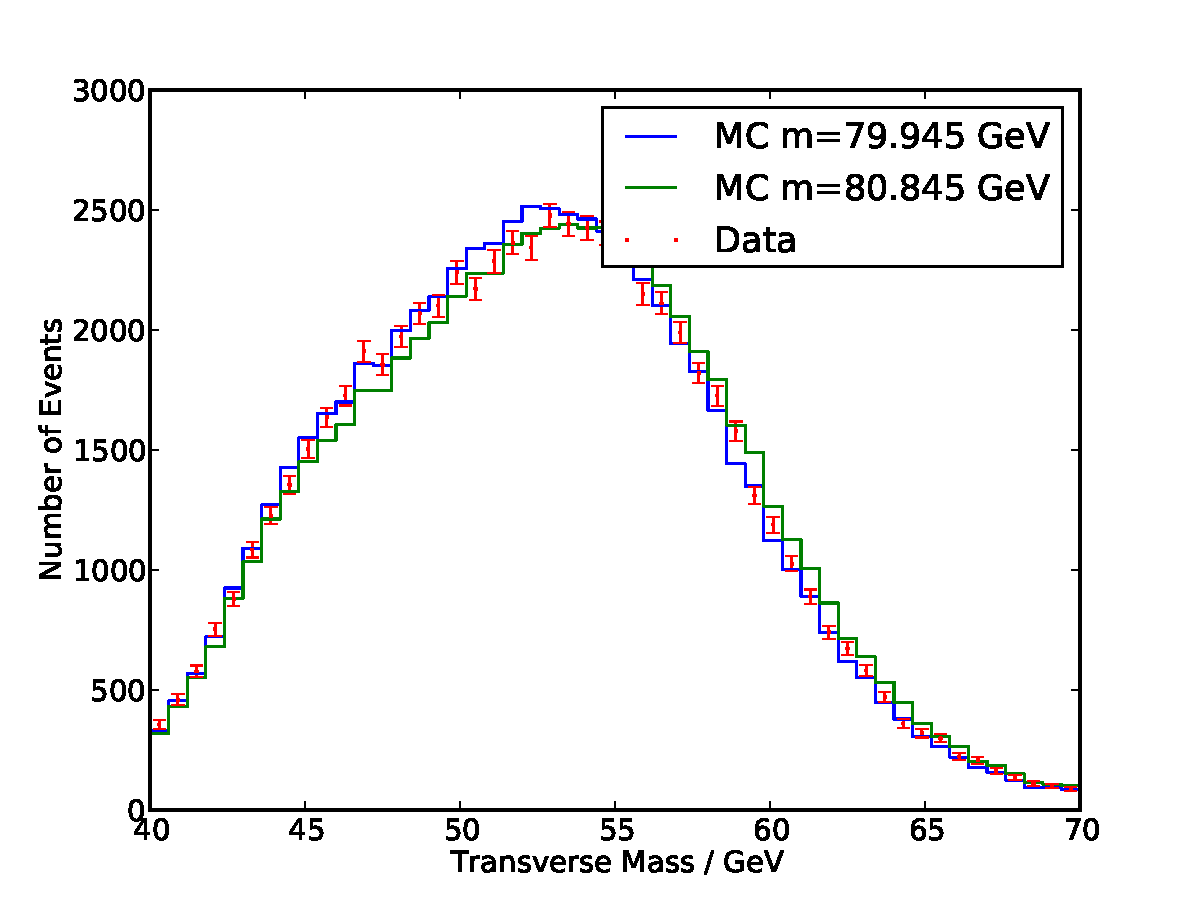
\includegraphics[width=0.8\textwidth]{comparison_m_t}
	\caption{Comparison of the transverse mass between data and MC with different input \PW boson masses.}
	\label{fig:comparison_m_t}
\end{figure}

The calculated $\chi^2$-values for each MC-set are presented in figure \ref{fig:chisquare_m_t}. In the minimum of the expected parabola, a $\chi^2 $ value of \num{68.0} is found. Together with the number of bins, this confirms the agreement between data and the MC set for this specific mass:
\begin{equation}
\frac{\chi^2}{n_{\mathrm{DoF}}} = \frac{\chi^2}{n_{\mathrm{bins}-1}} =  \frac{\num{68.0}}{\num{50} - \num{1}} \approx \num{1.39} 
\end{equation}

A fit of a parabolic function has been performed to find the best matching \PW mass. The fit range is chosen to the region around the minimum. The statistical error on the complete template method can then be obtained by intersecting the $\chi^2$-function with the horizontal line at $y=\chi^2_{\mathrm{min}}+1$. The final result of the minimization is stated in table \ref{tbl:m_results}.


\begin{figure}
	\centering
	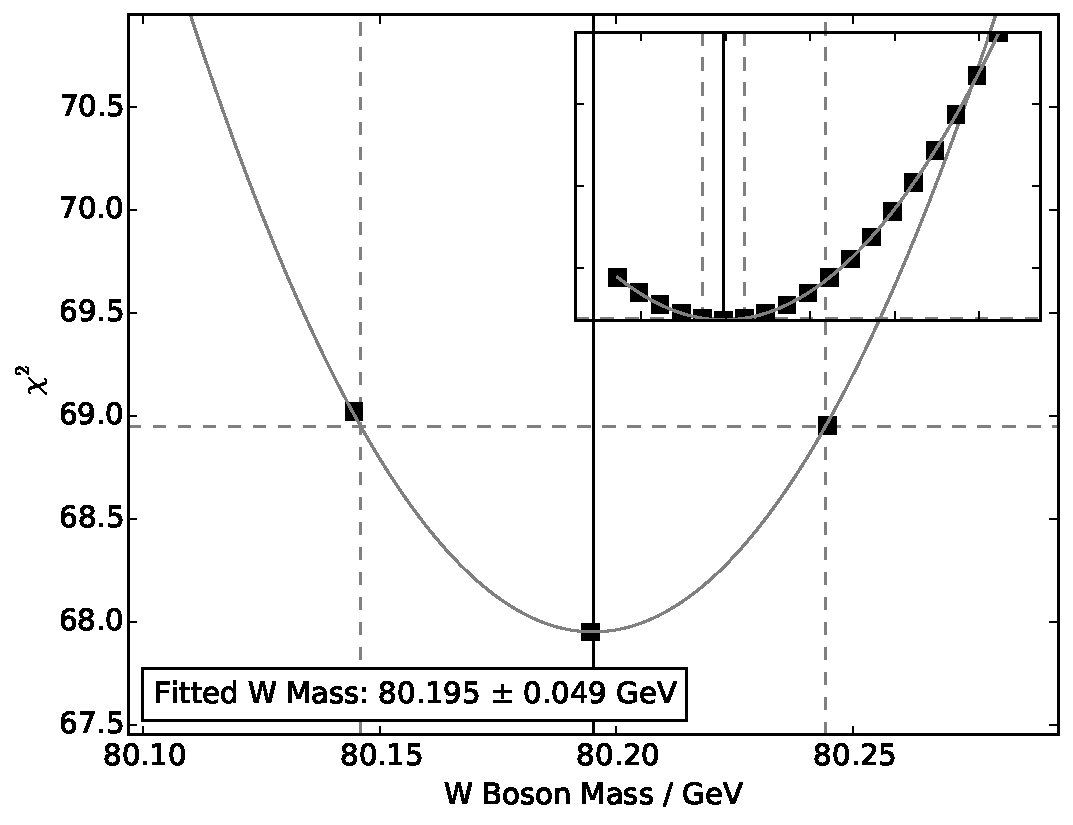
\includegraphics[width=0.8\textwidth]{chisquare_m_t}
	\caption{Result of the $\chi^2$ calculation for the 19 different \MT distributions compared to the dataset. The plot shows a zoom to the region around the minimum while all calculated points are presented in the small plot in the upper right corner. The dashed lines illustrate the estimation of the statistical error.}
	\label{fig:chisquare_m_t}
\end{figure}

\FloatBarrier

\subsection{Template Fit to the Transverse Electron Energy}
In almost the same manner as the distribution of \MT contains information on the \PW boson mass, it is also possible to investigate the distribution of the electron energy \ELET. The methods described above can be applied in the same way and the results are similar, see figures \ref{fig:comparison_el_et} and \ref{fig:chisquare_el_et}. However, the minimization of $\chi^2$ yields a slightly different value for \MW. This discrepancy will be discussed in the following sections.

\begin{figure}
	\centering
	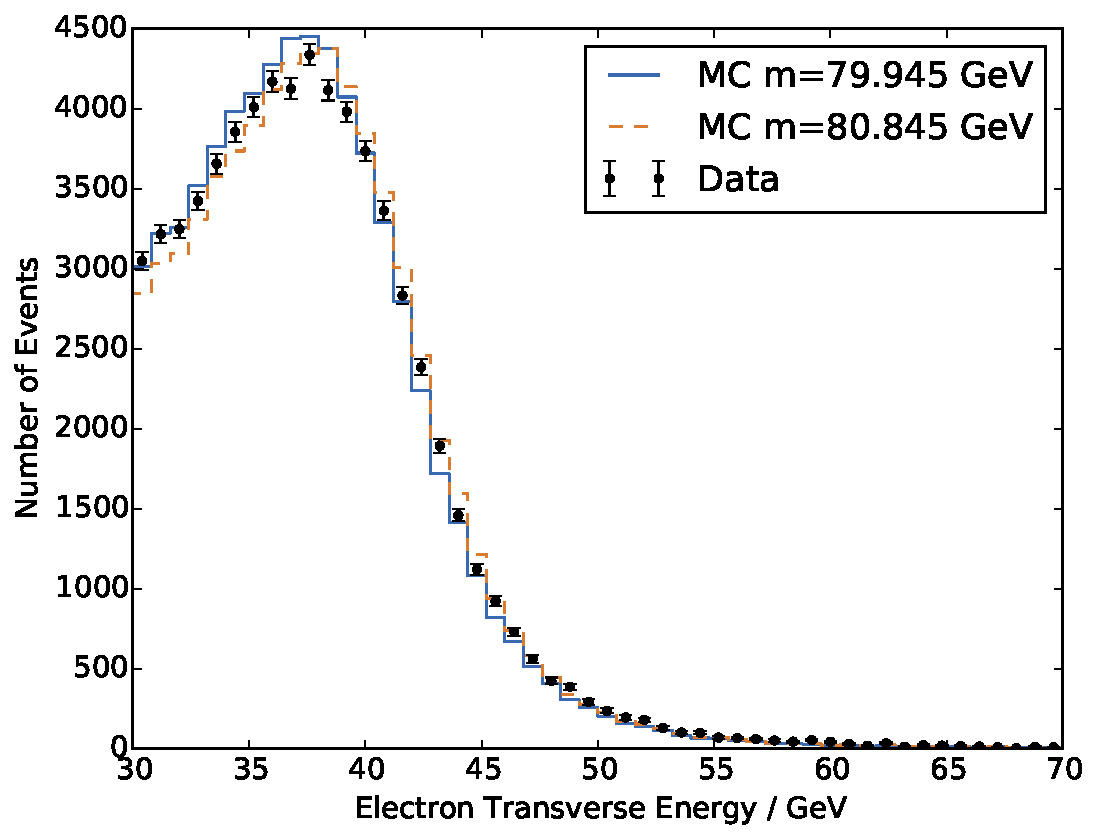
\includegraphics[width=0.8\textwidth]{comparison_el_e_t}
	\caption{Comparison of the transverse electron energy between data and MC with different input \PW boson masses.}
	\label{fig:comparison_el_et}
\end{figure}


\begin{figure}
	\centering
	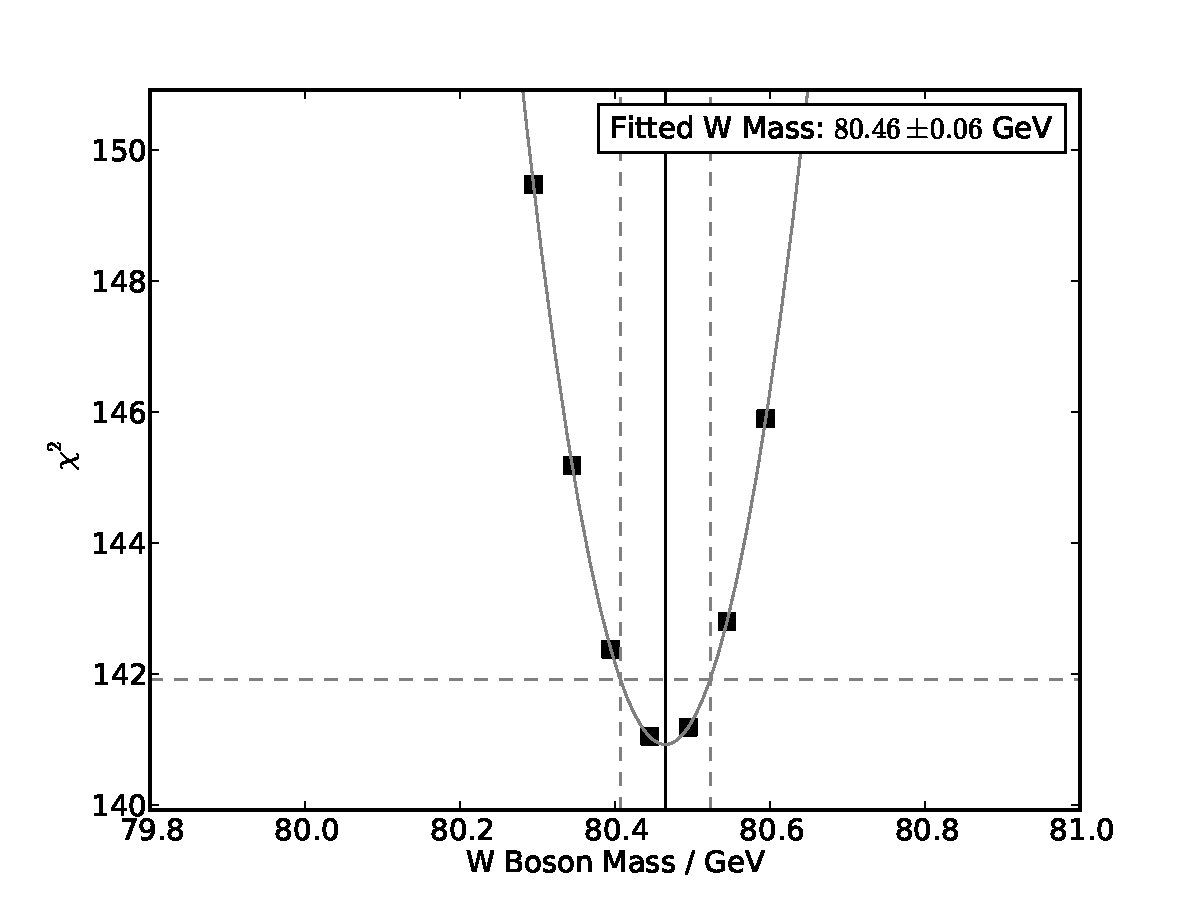
\includegraphics[width=0.8\textwidth]{chisquare_el_e_t}
	\caption{Result of the $\chi^2$ calculation for the 19 different \ELET distributions compared to the dataset.}
	\label{fig:chisquare_el_et}
\end{figure}

\FloatBarrier

\section{Systematic Uncertainties}
\subsection{Energy Resolution of the EM Calorimeter}
As a first contribution to the systematic uncertainty of the presented measurement, the energy resolution of the electromagnetic calorimeter is investigated. Since the method is highly depending on the measured transverse electron energy, it's precision is very important. The energy resolution can be parametrized as follows \cite{PhysRevLett.77.3309}, where $E$ is given in $\SI{}{\giga\electronvolt}$:
\begin{equation}
\frac{\sigma_E}{E} = \num{0.015} + \frac{\num{0.13}}{\sqrt{E}} + \frac{\num{0.4}}{E}
\label{eq:E_res}
\end{equation}
To estimate the impact of the limited resolution, the template fits are repeated 10 times but for each event the electron energy is smeared randomly following a gaussian distribution with $\sigma$ taken from equation \ref{eq:E_res}. This procedure results in 10 fitted \PW boson masses. The variance of this set is then taken as an estimator for the systematic uncertainty due to the energy resolution. The result is stated in table \ref{tbl:systematics}.

\subsection{Energy Scale Uncertainty of the EM Calorimeter}
\label{sec:sys_scale}
The energy scale of the electromagnetic calorimeter has been determined and parametrized by the \dnull collaboration \cite{PhysRevLett.77.3309} in decays of well-known particles of the standard model (e.g. $\pi^0$):
\begin{equation}
E_\mathrm{meas}= \alpha E + \delta
\end{equation}
However, this correction, which is applied to each event, contains uncertainties again. To investigate the impact of this systematic uncertainty, all measured electron energies are shifted once up and once down (no random process). The uncertainties on the two parameters are $\sigma_{\alpha} \approx 0.2 \%$ and $\sigma_{\delta} \approx 0.015$. This yields in the correction of $E_{\mathrm{meas}}$ a shift of:
\begin{equation}
E_\mathrm{meas}^\pm = E_\mathrm{meas} \pm ( \SI{0.2}{\percent} \cdot E_\mathrm{meas} + \num{0.015})
\end{equation}
The template fits are repeated and the impact of this fixed shift on the final result of \MW is investigated. Since this process is not stochastic, an estimator for the impact can be obtained as half of the width between the two shifted results:
\begin{equation}
\Delta \MW = \frac{\left|\MW\left(E_\mathrm{meas}^+\right) - \MW\left(E_\mathrm{meas}^-\right)\right|}{2}
\label{eq:sys_prop}
\end{equation} 
The determined uncertainties lie in the same order of magnitude as those from the energy resolution and can be found in table \ref{tbl:systematics}.

\subsection{Impact of the Cut Selection}
A third source of systematic uncertainties is the selection of cuts. Some of the cuts are motivated physically, some just to find a region of good agreement between MC and Data. However, another choice of cuts would have been possible as well. To estimate the impact of this ambiguity on \MW, the cuts are shifted separately in a reasonable range and the template fits are repeated. Similar to the explanation in section \ref{sec:sys_scale}, the uncertainty on the final result can then be estimated from equation \ref{eq:sys_prop}. The result of this procedure is shown in table \ref{tbl:sys_cuts}. Afterwards, the uncertainties are summed in quadrature (no correlation assumed).

\begin{table}[htbp]
	\centering
	\begin{tabular}{ 
			l 
			l
			S[table-format=3]
			S[table-format=3]
			}
		\toprule
		{Changed Cut} & {Shifted Range} & {$\Delta \MW(\MT)$ / \si{\mega\electronvolt}} & {$\Delta \MW(\ELET)$ / \si{\mega\electronvolt}} \\ 
		\midrule
		\MET & $\pm \SI{3}{\giga\electronvolt}$ & 26 & 3 \\
		\ELET & $\pm \SI{5}{\giga\electronvolt}$ & 25 & 58 \\
		Electron Isolation  & $\pm \num{0.01}$ & 72 & 91\\
		$\Delta \phi\left(\MET,\ELET\right)$ & $\pm \num{0.15}$ & 13 & 23\\ 
		$\Delta z\left(\MET,\ELET\right)$ & $\pm \num{0.05}$  &  1 & 8\\
		\midrule
		Total &  & 82 & 111 \\
		\bottomrule
	\end{tabular}
	\caption{Impact of the variation of the applied cuts on the \PW boson mass from the template fit. The last row contains the combined error, the uncertainties have been added in quadrature.}
	\label{tbl:sys_cuts}
\end{table}

All systematic uncertainties combined can be found in table \ref{tbl:systematics}.

\begin{table}[htbp]
	\centering
	\begin{tabular}{ 
			l
			S[table-format=3]
			S[table-format=3]
		}
		\toprule
		Systematic & {$\Delta \MW(\MT)$ / \si{\mega\electronvolt}} & {$\Delta \MW(\ELET)$ / \si{\mega\electronvolt}} \\ 
		\midrule
		Energy Resolution &  18 & 45 \\
		Energy Scale & 9 & 10  \\
		Cut Selection & 82 & 111  \\
		\midrule
		Total & 84 & 120 \\
		\bottomrule
		\end{tabular}
	\caption{Impact of the resolution smearing, rescaling within the energy scale uncertainty and variation of applied cuts on the \PW boson mass from the template fit. The combined error in the last row contains the values added in quadrature, since the choice of cuts, the energy scale and resolution are independent of each other.}
	\label{tbl:systematics}
\end{table}
One important source of systematic uncertainties is not considered yet: The measurement of the missing transverse energy. Since it is also based on the hadronic calorimeter, the fluctuations in the shower development and the lack of accurate hadronization models leads to a much larger uncertainty for \MET than for all measurements based on the electromagnetic calorimeter. However, to estimate this impact, precise information about the hadronic calorimeter and the coverage of the detector would be required. Therefore, this factor remains unknown in this analysis. 

\section{Results of the \PW Boson Mass Determination}

After combining the discussed uncertainties, the two template fits yield the following results: 
\begin{table}[htbp]
	\centering
	\begin{tabular}{ 
			l 
			l
			l
			l
		}
		\toprule
		{Investigated Quantity} & {\MW / \SI{}{\giga\electronvolt}} \\ 
		\midrule
		Transverse Mass \MT & $\num{80.195} \pm \num{0.049}_\mathrm{stat} \pm \num{0.084}_\mathrm{sys}$ \\
		Transverse Electron Energy \ELET & $\num{80.477} \pm \num{0.058}_\mathrm{stat} \pm \num{0.120}_\mathrm{sys}$\\
		\bottomrule
	\end{tabular}
	\caption{Determined \PW Boson mass from different template fits. The statistical error is solely taken from the $\chi^2$-fit, the systematic uncertainties are listed in tables \ref{tbl:sys_cuts} and \ref{tbl:systematics}.}
	\label{tbl:m_results}
\end{table}
\subsection{Combining the Determined Results - Correlation}
Although the determined results are compatible within their uncertainties, a combination is not trivial. As shown in figure \ref{fig:corr}, the transverse mass and the transverse electron energy are highly correlated. This was of course expected, since \MT depends linearly on \ELET, see equation \ref{eq:m_t}. Furthermore, the hard cut on the transverse electron energy becomes visible at $\ELET=\SI{30}{\giga\electronvolt}$. Quantitively, the correlation of the events in the dataset can be expressed in the correlation coefficient which is:
\begin{equation}
\rho (\MT,\ELET) = \num{0.886}
\end{equation}
\begin{figure}
	\centering
	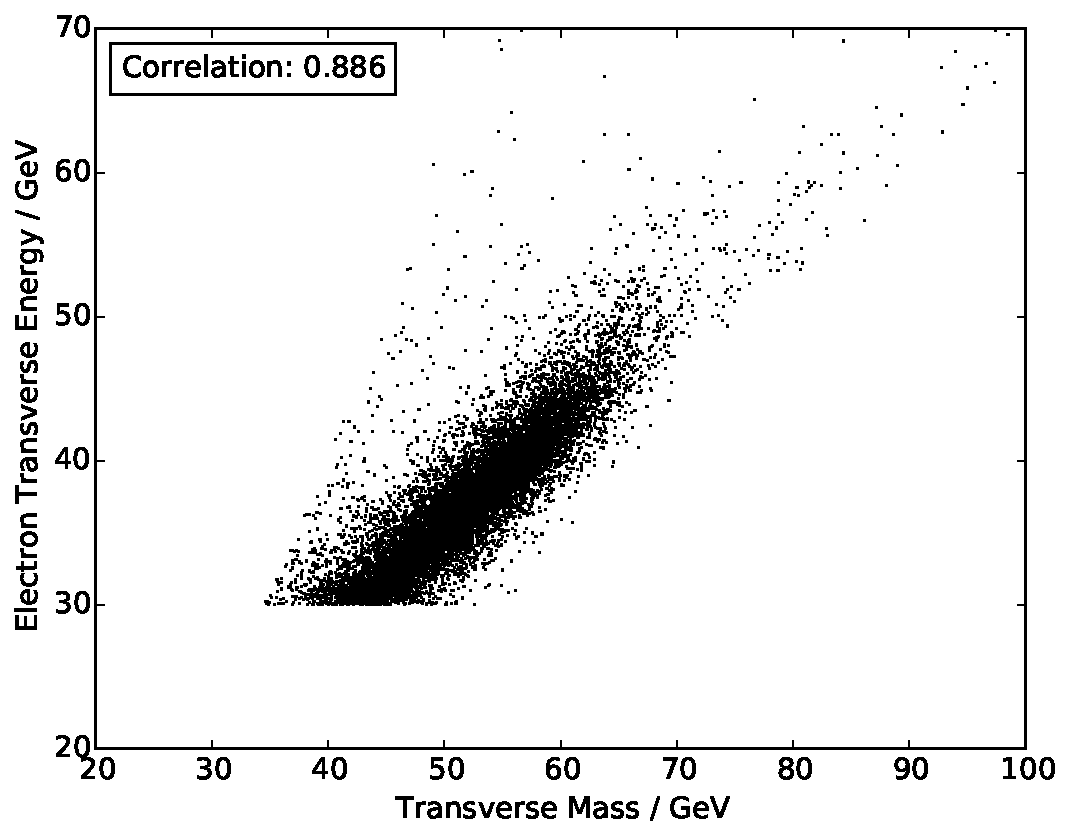
\includegraphics{correlation}
	\caption{Scatter plot of \MT vs. \ELET to illustrate the correlation between these quantities.}
	\label{fig:corr}
\end{figure}

\FloatBarrier

For the following analysis steps, the \PW mass determined in the template fit of the transverse electron energy is used. The reason lies in the unknown systematic uncertainty of the missing energy: Although the result from the fit of the transverse mass has slightly smaller uncertainties, the result from the fit of the electron energy is expected to be more precise if the uncertainty on the missing energy would be included. 

\begin{table}[htbp]
	\centering
	\begin{tabular}{ 
			l 
			l
			l
			l
		}
		\toprule
			 & {\MW / \SI{}{\giga\electronvolt}} \\ 
		\midrule
		This Analysis & $\num{80.477} \pm \num{0.058}_\mathrm{stat} \pm \num{0.120}_\mathrm{sys}$ \\
		World Average \cite{Oo2014Review} & $\num{80.385} \pm  \num{0.015}$ \\
		\bottomrule
	\end{tabular}
	\caption{Final result of the determined \PW boson mass.}
	\label{tbl:m_final}
\end{table}

Table \ref{tbl:m_final} shows the final result of this analysis in comparison with the World Average presented by the Particle Data Group. Within the estimated uncertainties, the two values are in good agreement.

\chapter{Sequential Calculations}

\section{Calculation of the Weak Mixing Angle}
The weak mixing angle, often also called Weinberg angle, describes a relation between the gauge boson masses in the Standard Model:
\begin{equation}
	\frac{\MW}{\MZ} = \cos \weinberg
\end{equation}

Combining the Particle Data Group's published mass of the \PZ boson\cite{Oo2014Review} with the measurement from this analysis, the mixing angle can be calculated
\begin{equation}
	\weinberg = \arccos \left( \frac{\MW}{\MZ} \right) = \arccos \left( \frac{\SI{80.477 +- 0.133}{\giga\electronvolt}}{\SI{91.1876 +- 0.0021}{\giga\electronvolt}} \right) = \SI{28.05 +- 0.18}{\degree}
\end{equation}
Here, the statistic and systematic uncertainties of this analysis' measurement have been combined by addition in quadrature, since they are assumed to be uncorrelated. Furthermore, Gaussian error propagation has been applied.

In the literature often mentioned is $\sin^2 \weinberg$, which consequently is
\begin{equation}
	\sin^2 \weinberg = 1 - \left( \frac{\MW}{\MZ} \right)^2 = \num{0.2211 +- 0.0026}
\end{equation}
This result is compatible with the literature value of $\sin^2 \weinberg = \num{0.22333}$\cite{Oo2014Review}, which also has been obtained by analyzing the \PW on-shell production. There are several other ways to measure the mixing angle, most results are a little larger (between \numrange{0.23126}{0.23864}) and not compatible with this measurement.

\section{Calculation of the Partial Decay Width}
The lab manual proposes a Standard Model equation describing the partial decay width of the \PW boson into fermions. Quark mixing, which is introduced by the CKM (Cabbibo-Kobayashi-Maskawa) matrix is neglected, thus a purely diagonal CKM matrix is assumed:
\begin{equation}
	\Gammaff = \frac{\alpha \cdot \MW}{12 \cdot \sin^2 \weinberg} = \SI{221.3 +- 2.9}{\giga\electronvolt}
\end{equation}
Here, the correlation between \MW and \weinberg has been considered and propagated onto the final result.

From this result, two subsequent calculations can be performed: one can either assume the Standard Model color factor of $\NC = \num{3}$ and calculate the total \PW decay width, or alternatively use literature decay width to calculate the color factor. Both approaches will be discussed in the following sections.

\section{Calculation of the Total Decay Width}
The total decay width of the \PW boson is assumed to contain equal contribution from all fermions, with the exception of the top and bottom quarks, which cannot be produced in the decay due to their higher mass. The partial decay width to quarks is additionally \NC times larger because they exist in \NC different colored versions.
\begin{equation}
	\GammaW = 3 \cdot \Gamma_\mathrm{\Plepton \Pnu} + 2 \cdot \Gamma_\mathrm{\Pquark \Pquark} = 3 \cdot \Gammaff + 2 \cdot \NC \cdot \Gammaff = \left( 3 + 2 \NC \right) \cdot \Gammaff
	\label{eq:total_decay_width}
\end{equation}

Using the Standard Model color factor of $\NC = \num{3}$, the total decay width is thus
\begin{equation}
	\GammaW = (3 + 2 \cdot 3) \Gammaff = \SI{1.991 +- 0.026}{\giga\electronvolt}
\end{equation}
This result is not compatible with the literature value of $\SI{2.085 +- 0.042}{\giga\electronvolt}$, and additionally has a smaller uncertainty. 

\section{Calculation of the Number of Colors}
As a second approach, the literature value for the total decay width is used and the number of colors is determined from it. This is basically using \ref{eq:total_decay_width}, solved for \NC:
\begin{equation}
	\NC = \frac{1}{2} \left( \frac{\GammaW}{\Gammaff} - 3 \right) = \num{3.21 +- 0.11}
\end{equation}
The Standard Model expectation $\NC = \num{3}$ has a distance of $2 \sigma$ to this measurement. But since the distance to $\NC = \num{2}$ or $\NC = \num{4}$ is larger, the Standard Model is still the favored hypothesis from this result.

\chapter{Conclusions}
\enlargethispage{0.5cm}
In this report, a measurement of the \PW boson mass has been presented together with the determination of the production and decay cross-section in electrons. Based on preselected data taken by the \dnull detector at the \Pproton\APproton -collider Tevatron, a template fit has been performed to extract \MW from the transverse electron energy measured in the electromagnetic calorimeter. The final result is 
\begin{equation}
	\MW = \SI[parse-numbers=false]{80.477 \pm 0.058_\mathrm{stat} \pm 0.120_\mathrm{sys}}{\giga\electronvolt}
\end{equation}
The statistical uncertainty coming from the $\chi^2$-minimization is much smaller than the systematic uncertainty which arises from the uncertainty in energy resolution and energy scale of the electromagnetic calorimeter as well as from the choice of cuts. An improvement on the precision of the analysis could be achieved by a more sophisticated Monte Carlo simulation: If for example the background processes was included in the simulated events, the analysis would be much less sensitive to the choice of cuts. The same holds for the uncertainties of the calorimeter measurement where the uncertainties could be included in the MC. Overall, the measurement of \MW stands in good agreement with the world average presented by the Particle Data Group and further quantities of the Standard Model could be computed sequentially.

\section{Advantages and Disadvantages of the Presented Analysis}
Proton-antiproton collisions e.g. at \dnull are well suited for the measurement of the \PW boson pole. \PW production and decay is a tree level process, and as such more probable than the \PW boson production at the Large Electron Positron collider (LEP) via the process $\Pelectron + \Ppositron \rightarrow \PZ \rightarrow \PWplus + \PWminus \rightarrow ...$.
Thus, the event yield at \dnull is much larger than at the LEP experiments. A disadvantage is that due to protons being composite particles, the center of mass energy of the collision is unknown and all measurements have to be performed in the two-dimensional transversal plane. In an experiment which collides elementary particles, such as electrons and positrons at LEP, the full three-dimensional information can be used to reconstruct the \PW mass. On the other hand, due to the lower statistics, also hadronic final states are an important part of \PW boson measurements at LEP. This introduces other complications, for example Bose-Einstein-Correlations between the produced hadrons in the outgoing jets \cite{Kress:2002hb}. 

\cleardoublepage

\bibliographystyle{utphys}
\bibliography{T17_bib}{}



\end{document}
